\documentclass{sigchi}

% Load basic packages
\usepackage{balance}       % to better equalize the last page
\usepackage{graphics}      % for EPS, load graphicx instead
\usepackage[T1]{fontenc}   % for umlauts and other diaeresis
\usepackage{txfonts}
\usepackage{mathptmx}
\usepackage[pdflang={en-US},pdftex]{hyperref}
\usepackage{color}
\usepackage{booktabs}
\usepackage{textcomp}

% Some optional stuff you might like/need.
\usepackage{microtype}        % Improved Tracking and Kerning
% \usepackage[all]{hypcap}    % Fixes bug in hyperref caption linking
\usepackage{ccicons}          % Cite your images correctly!
% \usepackage[utf8]{inputenc} % for a UTF8 editor only

% Paper metadata (use plain text, for PDF inclusion and later
% re-using, if desired).  Use \emtpyauthor when submitting for review
% so you remain anonymous.
\def\plaintitle{Physical Effort and Expressivity in\\ Digital Musical Instruments}
\def\plainauthor{Tom Gurion}
\def\plainkeywords{Effort; Expression; Digital musical instruments.}

% llt: Define a global style for URLs, rather that the default one
\makeatletter
\def\url@leostyle{%
  \@ifundefined{selectfont}{
    \def\UrlFont{\sf}
  }{
    \def\UrlFont{\small\bf\ttfamily}
  }}
\makeatother
\urlstyle{leo}

% To make various LaTeX processors do the right thing with page size.
\def\pprw{8.5in}
\def\pprh{11in}
\special{papersize=\pprw,\pprh}
\setlength{\paperwidth}{\pprw}
\setlength{\paperheight}{\pprh}
\setlength{\pdfpagewidth}{\pprw}
\setlength{\pdfpageheight}{\pprh}

% Make sure hyperref comes last of your loaded packages, to give it a
% fighting chance of not being over-written, since its job is to
% redefine many LaTeX commands.
\definecolor{linkColor}{RGB}{6,125,233}
\hypersetup{%
  pdftitle={\plaintitle},
  pdfauthor={\plainauthor},
  pdfkeywords={\plainkeywords},
  pdfdisplaydoctitle=true, % For Accessibility
  bookmarksnumbered,
  pdfstartview={FitH},
  colorlinks,
  citecolor=black,
  filecolor=black,
  linkcolor=black,
  urlcolor=linkColor,
  breaklinks=true,
  hypertexnames=false
}

% create a shortcut to typeset table headings
% \newcommand\tabhead[1]{\small\textbf{#1}}

% End of preamble. Here it comes the document.
\begin{document}

\title{\plaintitle}

\numberofauthors{1}
\author{%
  \alignauthor{Tom Gurion\\
    \affaddr{Media and Arts Technology}\\
    \affaddr{Queen Mary University of London}\\
    \email{t.gurion@qmul.ac.uk}}\\
}

\maketitle

% TODO abstract
\begin{abstract}
  Lorem ipsum dolor sit amet, consectetur adipisicing elit, sed do eiusmod tempor incididunt ut labore et dolore magna aliqua. Ut enim ad minim veniam, quis nostrud exercitation ullamco laboris nisi ut aliquip ex ea commodo consequat. Duis aute irure dolor in reprehenderit in voluptate velit esse cillum dolore eu fugiat nulla pariatur. Excepteur sint occaecat cupidatat non proident, sunt in culpa qui officia deserunt mollit anim id est laborum.
\end{abstract}

\keywords{\plainkeywords}

\section{Introduction}

The use of computers and digital instruments is common in nowadays musical performances.
One significant different between traditional and digital musical instruments performances is that physical effort is usually involve in the former, but can be totally absent in the later.
This difference presents several issues for live computer music.
For example, it might prevent the audience from understanding the performance.
On the extreme, the listener might question the "liveness" of a performance altogether when he can't tell the difference between live and pre-composed playback.
Besides, visible effort is an important expressive tool in many musical contexts.
TODO BETTER EXAMPLES
Consider, for example, a trumpet player and his outcurved veins in the neck while he reaches a high note, or a drummer, sweating during intense performance.

TODO Define the issue better. Digital musical instruments are not laptop music, but some of the issues overlap.

Theoretical studies from the last few decades highlited these issues.
Some researchers explain the core of the problem by the lack of apparant relationship between the way an instrument is played and the resulted sound \cite{Schloss2003,DEscrivan2006}.
Others argue that computers promote "effortless interaction" and by that contradict they way music should be created \cite{Ryan1992}.
Most of the research in the field, however, doesn't confront the theoretical hypotheses using rigrous experiments.
One exception is a recent experiment based study by Bown et al.\ \cite{Bown2014}.
Their results show that listeners do able to perceive what the performer is doing from the audio alone.

Along with these lines, the current study examines to what extent physical effort can enhance expressivity in playing digital instruments.
In addition, it explores the effect of the performer's physical effort on the audience perception and appreciation of the performance.
These questions are assessed in controlled experiment, evaluating perceived expressivity from the point of view of the performer and the listener alike.

The current work uses the Schleikess interface, a digital controller for interactive performance that requires physical effort and large body movements from the performer, to assess performance expressivity.
Figure \ref{fig:schleikess} shows a schematic diagram of the interface.
It is composed of two elastic bands, each of them is connected with one side, through a load sensor, to the belt loop of the performer.
The performer holds the other side of the elasic bands and can strech them to play.

This controller can be used for different creative purposes.
In the context of this study one elastic band controls the pitch and the other controls the amplitude of a sawtooth tone generator.
TODO discuss more this type of interaction. Simple relationship between gestures and produced sound helps the audience to understand the performance. TODO search and reference the theramin design decition.

\begin{figure}
  \centering
  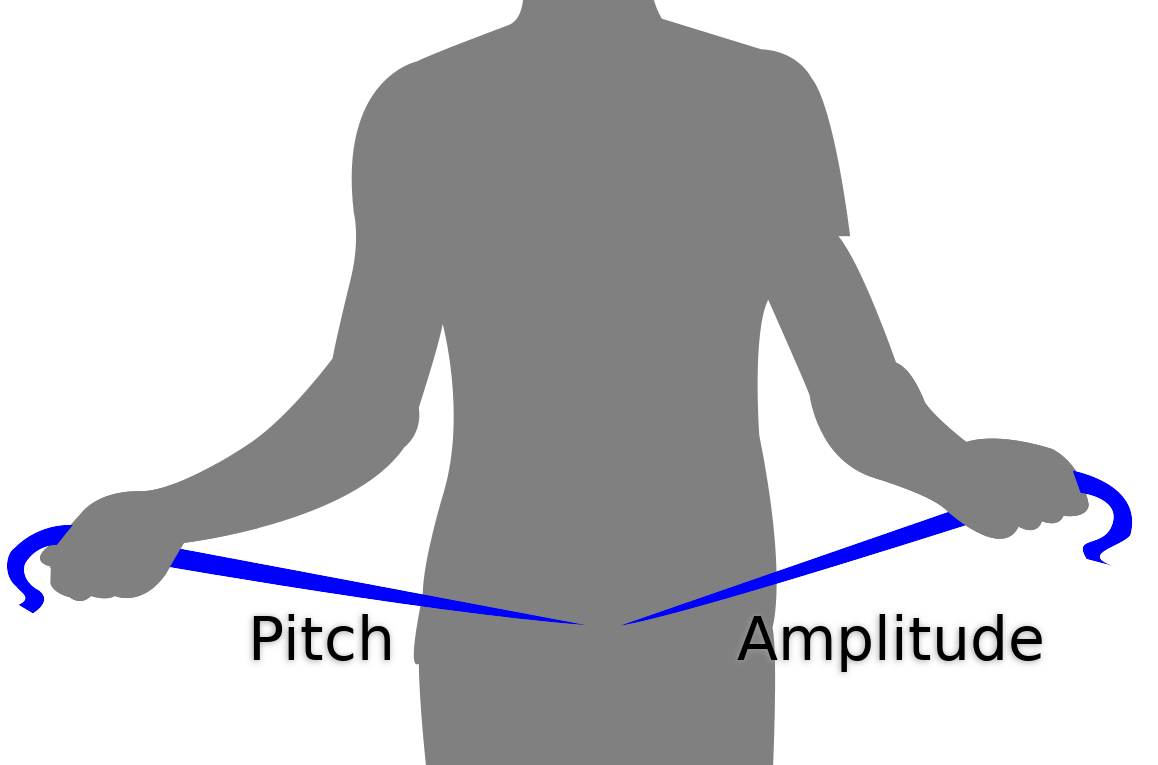
\includegraphics[width=0.9\columnwidth]{figures/schleikess}
  \caption{A diagram of the Schleikess interface. In blue are the two elastic bands. Stretching the left raises the pitch and stretching the right raises the amplitude.}~\label{fig:schleikess}
\end{figure}

\section{Initial study}

\subsection{Methods}

In an initial study I examined to what extent physical effort can enhance expressivity in playing digital instruments.
TODO X participants were invited to play with the Schleikess based synthesiser and discuss their subjective experience.
Apart from playing, they could modify the amount of physical effort required by the instrument by changing the sensitivity of the interface to force.
Two sliders on the computer screen controlled the sensitivity, one for the pitch and one for the amplitude.
This way, when the sensitivity is low, a major physical force is needed to raise the pitch or amplitude, but when the sensitivity was high even minor changes affect the output significantly.
The participants were instructed that they need to stretch the elastic bands to play the instrument and that the sliders on the computer screen changes the sensitivity of the instrument.
However, the relationship between stretching the bands and the resulted sound was not explaind.

The participants were asked to familiarize themeselves with the instrument, understand the mapping between gestures and sound, and then set the sliders to the values they find most expressive.
Later, I discussed with each participant about the experience of playing the instrument.
The discussion concentrated around questions of how expressive and musical the instrument felt with differente sensitivity settings.

This type of exploratory initial study is designed to get basic insights about the relationships between physical effort and expressivity.
Provided that there is almost no empirical research in this field, this type of broad exploration is necessary to gain first insights.

\subsection{Results}

Lorem ipsum dolor sit amet, consectetur adipisicing elit, sed do eiusmod tempor incididunt ut labore et dolore magna aliqua. Ut enim ad minim veniam, quis nostrud exercitation ullamco laboris nisi ut aliquip ex ea commodo consequat. Duis aute irure dolor in reprehenderit in voluptate velit esse cillum dolore eu fugiat nulla pariatur. Excepteur sint occaecat cupidatat non proident, sunt in culpa qui officia deserunt mollit anim id est laborum.

\section{Discussion}

Lorem ipsum dolor sit amet, consectetur adipisicing elit, sed do eiusmod tempor incididunt ut labore et dolore magna aliqua. Ut enim ad minim veniam, quis nostrud exercitation ullamco laboris nisi ut aliquip ex ea commodo consequat. Duis aute irure dolor in reprehenderit in voluptate velit esse cillum dolore eu fugiat nulla pariatur. Excepteur sint occaecat cupidatat non proident, sunt in culpa qui officia deserunt mollit anim id est laborum.

\subsection{Future research}

Lorem ipsum dolor sit amet, consectetur adipisicing elit, sed do eiusmod tempor incididunt ut labore et dolore magna aliqua. Ut enim ad minim veniam, quis nostrud exercitation ullamco laboris nisi ut aliquip ex ea commodo consequat. Duis aute irure dolor in reprehenderit in voluptate velit esse cillum dolore eu fugiat nulla pariatur. Excepteur sint occaecat cupidatat non proident, sunt in culpa qui officia deserunt mollit anim id est laborum.

% BALANCE COLUMNS
\balance{}

% REFERENCES FORMAT
% References must be the same font size as other body text.
\bibliographystyle{SIGCHI-Reference-Format}
\bibliography{bib}

\end{document}

%%% Local Variables:
%%% mode: latex
%%% TeX-master: t
%%% End:
